\documentclass[a4paper,9pt]{article}

\usepackage[utf8]{inputenc}
\usepackage{graphicx}
\usepackage[francais]{babel}
%\usepackage{fullpage}
\usepackage{color}
\usepackage{array}

\begin{document}


\begin{titlepage}
\centering
\huge
\bfseries
Visualisation Scientifique\\[1\baselineskip]
\vspace{0.5cm}
\normalfont
\large
Interpolation et Visualisation de données avec Paraview\\[1\baselineskip]
	
\vspace{2cm}

\begin{figure}[!h]
\centering
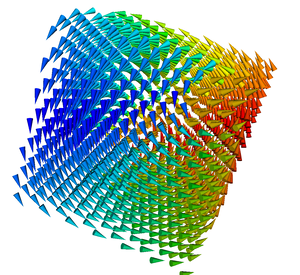
\includegraphics[width=0.9\textwidth]{couverture.png}
\end{figure}

\vspace{1.5cm}

\centering
\bfseries
\normalfont

\begin{tabular}{r c l}
Benjamin Aupetit & & Nicolas Cousin
\end{tabular}	

\vspace{0.5cm}

Ensimag\\
\textbf{\today}
\end{titlepage}

\clearpage
\newpage

\tableofcontents

\clearpage
\newpage

% INTRODUCTION

\section{Introduction}
\label{sec:introduction}
Une des étapes cruciales pour l'observation d'un phénomène a toujours été de prendre des séries de mesures des données physiques associées à ce phénomène. Malheureusement, il n'est pas toujours possible de mesurer une quantité en n'importe quel point de l'espace, d'abord parce que ça coûte cher et d'autre part parce que la position où l'on souhaite faire la mesure n'est pas toujours accessible.\\ Par conséquent, il existe des méthodes d'interpolation permettant d'évaluer approximativement la valeur d'une donnée physique (température, densité, ...) en un point de l'espace en fonction des valeurs que l'on a mesuré sur des positions voisines. Ce document présente deux méthodes d'interpolation que nous avons implémenté, et nous proposons ensuite de visualiser leurs résultats sur paraview qui est un logiciel permettant de visualiser les données d'une grille régulière.

\clearpage
\newpage

\section{Première Méthode : Shepard}
\label{sec:shepard}

\subsection{Description}
\label{subsec:shepard_description}
Le principe de cette méthode est de considérer que la valeur interpolée en une position de l'espace est une somme pondérée des valeurs des échantillons en entrée.
$$F(x)=\sum_{i=1}^{N} \omega_{i}(x).f_{i}$$
Chaque fonction de pondération $\omega_{i}$ est définie de la façon suivante :
$$\omega_{i}(x)=\frac{\prod_{j \neq i}^{N}[d_{j}(x)]^{\mu}}{\sum_{j=1}^{N} \prod_{k \neq j}^{N}[d_{k}(x)]^{\mu}} ~~~~~~ d_{i}(x)=||x-x_{i}||_{2}~~~,~~~\mu\ge1$$

\subsection{Complexité}
\label{subsec:shepard_complexite}
Notons $N$ le nombre d'échantillons de données en entrée et $R$ le produit des résolutions de la grille voulue :
$$R = resolution_{x}.resolution_{y}.resolution_{z}$$
La méthode de Shepard revient à multiplier deux matrices, l'une de taille $N.R$ qui contiendra à chaque ligne les différentes valeurs des coefficients $\omega_{i}$ pour un point de la grille, et l'autre étant le vecteur colonne de taille $N$ contenant les valeurs scalaires des échantillons en entrée. Le résultat de cette multiplication donne un vecteur colonne de taille $R$ contenant les $R$ valeurs scalaires interpolées pour les points de la grille.
$$S_{N,R}.F_{1,N}=Res_{1,R}$$
Le coût en calcul de cette méthode est donc la somme du coût pour construire la matrice S et le coût de la multiplication entre S et F.\\\\
\textbf{Coût de la construction de S}\\
Chaque coefficient de la matrice correspond au calcul d'un $\omega_{i}$ :
\begin{itemize}
\item Le coût de calcul du numérateur est en $O(N)$ mais doit être calculé pour chaque colonne d'une ligne de S
\item Le coût de calcul du dénominateur est en $O(N^{2})$ et peut être calculé une fois pour chaque ligne de S
\end{itemize}
Comme S a une largeur de $N$ et une hauteur de $R$, son coût de construction est donc en $O(N^{2}.R)$.\\\\
\textbf{Coût de la multiplication de S et F}\\
Etant donné la taille des matrices, son coût est en $O(N.R)$.\\\\
Par conséquent la méthode de Shepard a une complexité en \textbf{$O(N^{2}.R)$}.


\section{Deuxième Méthode : Multiquadriques de Hardy}
\label{sec:hardy}

\subsection{Description}
\label{subsec:hardy_description}

\subsection{Complexité}
\label{subsec:hardy_complexite}

\section{Implémentation}
\label{sec:implementation}

\subsection{Types utilisés}
\label{subsec:types}

\subsection{Implémentation de la méthode de Shepard}
\label{subsec:shepard_implementation}

\subsection{Implémentation de la méthode des multiquadriques de Hardy}
\label{subsec:hardy_implementation}

\section{Tests et Résultats}
\label{sec:tests_resultats}

\subsection{Visualisation de données avec Paraview}
\label{subsec:paraview}

\subsection{Présentation des méthodes de tests}
\label{subsec:presentation_tests}

\subsection{Validation de l'implémentation}
\label{subsec:validation_implementation}

\subsection{Tests Complexes}
\label{subsec:tests_complexes}

\subsection{Comparaison des deux méthodes]}
\label{subsec:comparaison_methodes}

\subsubsection{Temps de calcul}
\label{subsec:temps_calcul}

\subsubsection{Précision de l'interpolation}
\label{subsec:precision_interpolation}

\section{Conclusion}
\label{sec:conclusion}

\end{document}
